\chapter{Experiments and Results}
\label{experiment}

\TG{Add a sentence or two summarizing what's in this chapter.}

\section{Experiments}

Our experiments compared real executions with our Python prototype, with the 
original \wrench simulator, and with our \wrench-cache extension. 
Executions included single-threaded and multi-threaded applications, 
accessing data on local and network file systems. 
We used two applications: a synthetic one, created to evaluate the simulation model, 
and a real one, representative of neuroimaging data processing.

Experiments were run on a dedicated cluster at Concordia University, with one 
login node, 9 compute nodes, and 4 storage nodes connected with a 25 Gbps network. 
Eachcompute node had 2 $\times$ 16-core Intel(R) Xeon(R) Gold 6130 CPU @ 2.10GHz, 
250~GiB of RAM, 6 $\times$ SSDs of 450~GiB each with the XFS file system, 
378~GiB of tmpfs, 126~GiB of devtmpfs file system, CentOS~8.1 and NFS version 4. 
We used the \texttt{atop} and \texttt{collectl} tools to monitor and collect memory status
and disk throughput. 
We cleared the page cache before each application run to ensure comparable conditions.
    
The synthetic application, implemented in C, consisted of three single-core,
sequential tasks where each task read the file produced by the previous task, 
incremented every byte of this file to emulate real processing, 
and wrote the resulting data to disk. 
Files were numbered by ascending access times (File 1 and File 2 were the files 
read and written respectively by Task 1, etc).
The anonymous memory used by the application was released after each task, 
an this memory release is also simulated in the Python prototype and 
in WRENCH-cache. 
As our focus was on I/O rather than compute, we measured CPU times 
of application tasks on a cluster node (Table~\ref{table:cputime}), and 
used these durations in our simulations. 
For the Python prototype, as we put a sleep time simulated tasks to 
simulate CPU time, we simply injected CPU times directly in the simulation. 
In \wrench, it simulates CPU time with the number of flops of tasks 
and the CPU speed of hosts.
Thus, for \wrench and \wrench-cache, we determined the corresponding 
number of flops on a 1~Gflops CPU and used these values in the simulation. 
The simulated the platform and application are available at commit 
\href{https://github.com/wrench-project/wrench/tree/ec6b43561b95977002258c0fe37a4ecad8f1d33f/examples/basic-examples/io-pagecache}{ec6b43561b}.

\begin{table}[!h]
    \centering
    \begin{tabularx}{0.8\columnwidth}{c>{\centering\arraybackslash}X}
    \toprule
        Input size (GB)  & CPU time (s)\\
    \midrule
        3 & 4.4 \\
        20  & 28 \\
        50  & 75 \\
        75  & 110 \\
        100  & 155 \\
    \bottomrule
    \end{tabularx}
    \caption{Synthetic application parameters}
    \label{table:cputime}
\end{table}

We used the synthetic application in three experiments. In the first one 
(\textit{Exp~1}), we ran \emph{a single instance} of the application on a 
single cluster node, with different input file sizes (20~GB, 50~GB, 75~GB, 100~GB), 
and with all I/Os directed to the same local disk.
The information about free memory, amount of dirty data, amount of cache used 
and free memory is collected using \texttt{atop} tool during the execution 
time of the tasks. We also used \texttt{fincore} to after each I/O operation 
to inspect the cache content with the amount of cached data of each file.  

In the second experiment (\textit{Exp~2}), we ran \emph{concurrent} instances 
of the application on a single node, all application instances operating on 
different files stored in the same local disk. Due to the limited capacity of 
the disk used, we used the file size of 3~GB. 
We varied the number of concurrent application instances from 1 to 32 
since cluster nodes had 32 CPU cores.
The read time, CPU time and write time of each instance were logged into 
log files. 

In the third experiment (\textit{Exp~3}), we used the same configuration as 
the previous one, albeit reading and writing on a 50-GiB NFS-mounted 
partition of a 450-GiB remote disk of another compute node. 
As is commonly configured in HPC environments to avoid data loss, 
there was no client write cache and the server cache was configured as 
writethrough instead of writeback. 
NFS client and server read caches were enabled. 
Therefore, all the writes happened at disk bandwidth, but reads could 
benefit from cache hits.

The real application was a workflow of the Nighres 
toolbox~\cite{huntenburg2018nighres}, implementing cortical reconstruction 
from brain images in four steps: skull stripping, tissue classification, 
region extraction, and cortical reconstruction. 
Each step read files produced by the previous step, and wrote files that 
were or were not read by the subsequent step.
More information on this application is available in the Nighres
documentation at
\url{https://nighres.readthedocs.io/en/latest/auto_examples/example_02_cortical_depth_estimation.html}.
The application is implemented as a Python script that calls Java
image-processing routines. We used Python 3.6, Java 8, and Nighres 1.3.0. 
In Nighres, data is read lazily and written in compressed format.
Thus, we patched the application to remove lazy data loading and data compression, 
which made CPU time difficult to separate from I/O time, and to capture task 
CPU times to inject them in the simulation. 
The patched code is available at \url{https://github.com/dohoangdzung/nighres}.

We used the real application in the fourth experiment (\textit{Exp~4}), 
run on a single cluster node using a single local disk. 
We processed data from participant 0027430 in the dataset of the 
Max Planck Institute for Human Cognitive and Brain Sciences available at
\url{http://dx.doi.org/10.15387/fcp_indi.corr.mpg1}, 
leading to the parameters in Table~\ref{table:nighres_stats}.

\begin{table}[!h]
    \centering
    \begin{tabular}{lccc}
    \toprule
        \multicolumn{1}{c}{Workflow step}& Input size       & Output size      & CPU time\\
                               & (MB)             & (MB)             & (s)\\
    \midrule
       Skull stripping         &  295             & 393               & 137 \\
       Tissue classification   &  197              & 1376              & 614 \\
       Region extraction       &  1376             & 885              & 76 \\
       Cortical reconstruction &  393              & 786              & 272\\
    \bottomrule
    \end{tabular} 
    \caption{Nighres application parameters}
    \label{table:nighres_stats}
\end{table}

To parameterize the simulators, we benchmarked the memory, local disk, 
remote disk (NFS), and network bandwidths (Table~\ref{table:benchmark}). 
Since \simgrid, and thus \wrench, currently only supports symmetrical 
bandwidths, we use the mean of the read and write bandwidth values 
in our experiments.

\begin{table}[!h]
        \centering
        \begin{tabularx}{\columnwidth}{ll
        >{\centering\arraybackslash}X
        >{\centering\arraybackslash}X
        >{\centering\arraybackslash}X}
        \toprule
            \multicolumn{2}{c}{Bandwidths}  & Cluster (real) & Python prototype & \wrench simulator\\
        \midrule
        \multirow{2}{*}{Memory}      & read  & 6860 & 4812 & 4812\\
                                     & write & 2764 & 4812 & 4812\\
        \multirow{2}{*}{Local disk}  & read  & 510  & 465  & 465\\
                                     & write & 420  & 465  & 465\\
        \multirow{2}{*}{Remote disk} & read  & 515  & -    & 445\\
                                     & write & 375  & -    & 445\\
        \multicolumn{2}{l}{Network}  & 3000  & -    & 3000\\
        \bottomrule
    \end{tabularx}
    \caption{Bandwidth benchmarks (MBps) and simulator configurations.
    The bandwidths used in the simulations were the average of the measured read and write bandwidths.
    Network accesses were not simulated in the Python prototype.}
    \label{table:benchmark}
\end{table}

% Finally, because \wrench simulates applications base on network-communication,
% we use an infinite bandwidth to eliminate network latency for local I/Os.

\section{Results}

\subsection{Single-threaded execution (Exp 1)}

\begin{figure*}[!h]
     \centering
     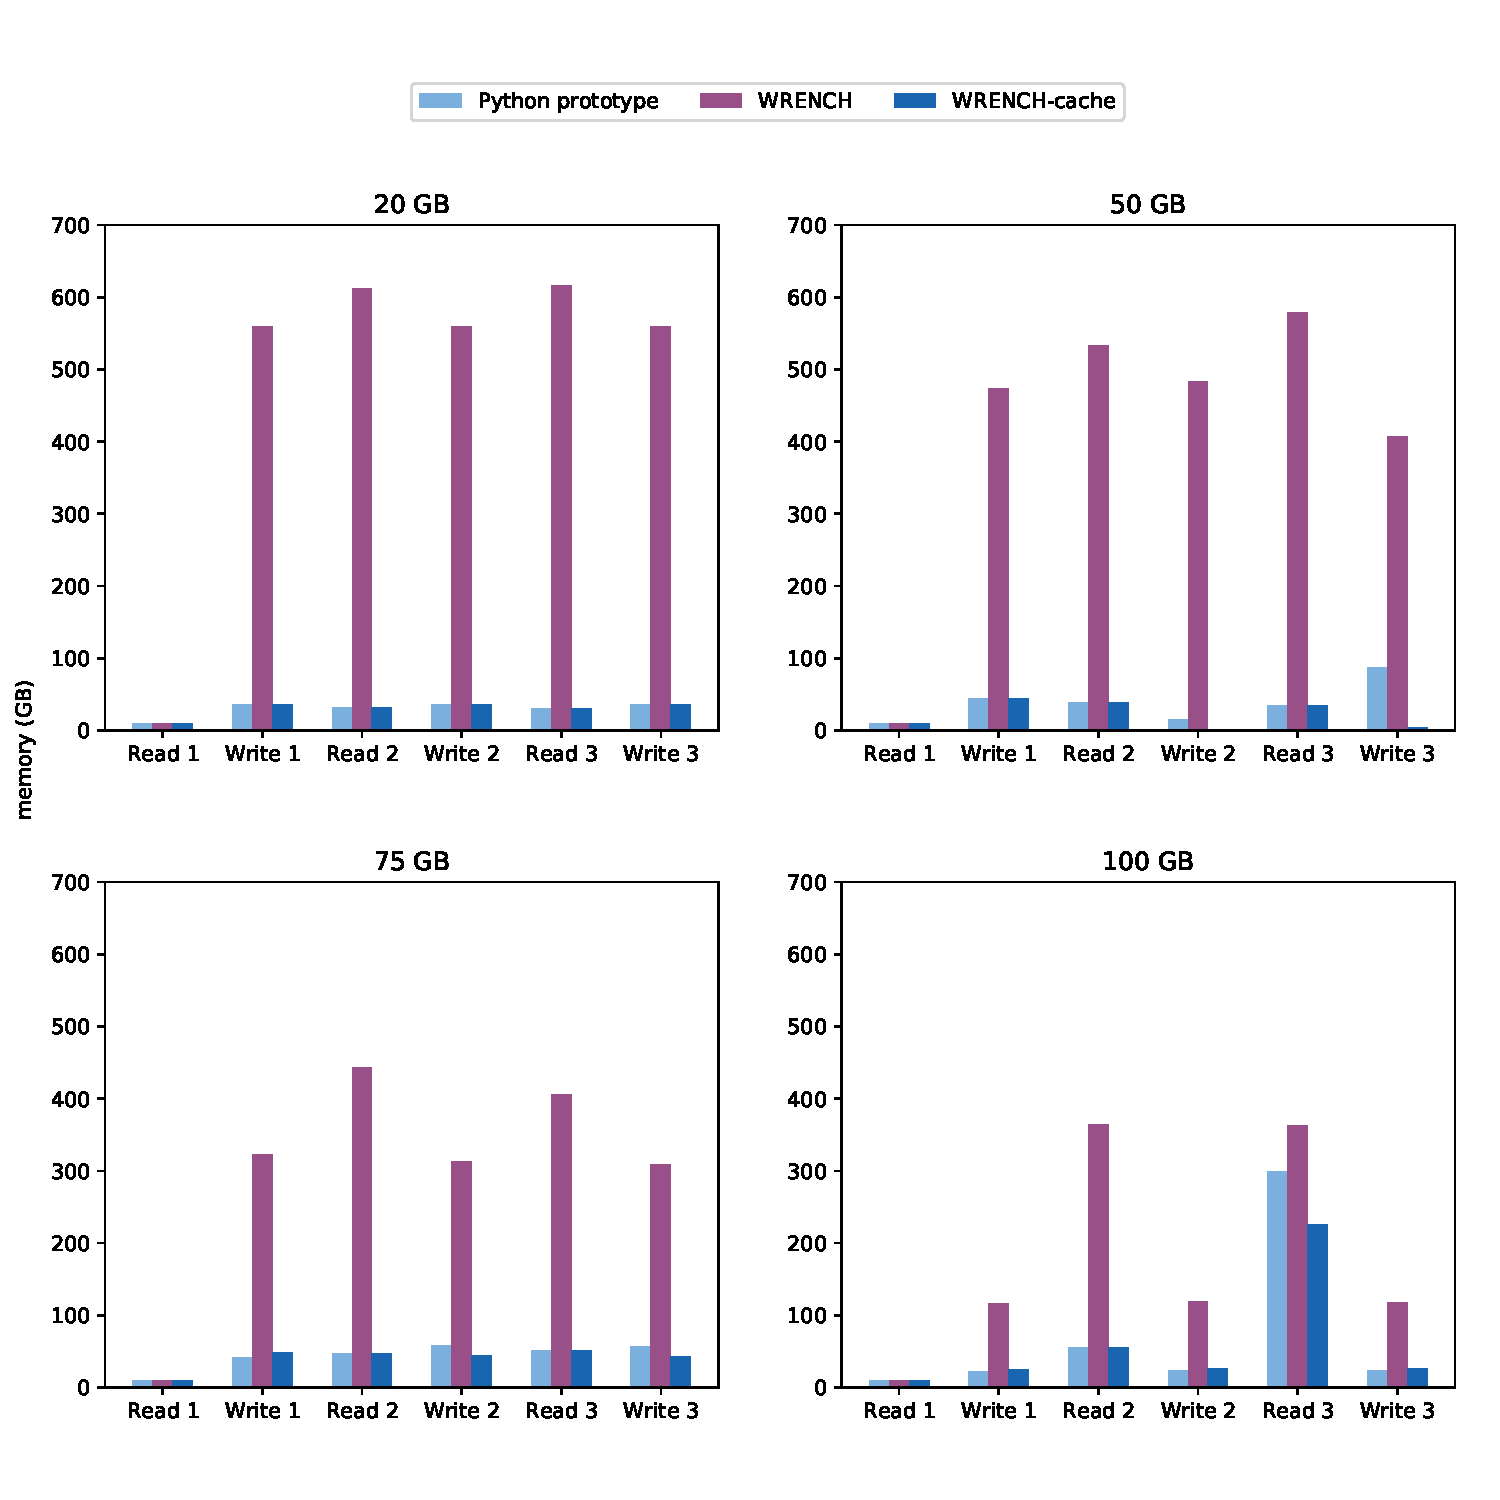
\includegraphics[width=\linewidth]{figures/single_errors_full.pdf}
%     \vspace*{-0.7cm}
     \caption{Absolute relative simulation errors of single-threaded application 
     with different file sizes}
%     \vspace*{0.5cm}
     \label{fig:single_error}
\end{figure*}

The page cache simulation model drastically reduced I/O simulation
errors in each application task (Figure~\ref{fig:single_error}). 
The first read was not impacted as it only involved uncached data. 
Errors were reduced from an average of 345\% in the original 
\wrench to 46\% in the Python prototype and 39\% in \wrench-cache. 
Unsurprisingly, the original \wrench simulator significantly overestimated 
read and write times, due to the lack of page cache simulation. 

As is shown in Figure~\ref{fig:single_error}, \wrench simulation errors 
substantially decreased as the input file size increased. 
This is due to the fact that as the input file size grew larger than a specific 
threshold in the experiment, all files can not fit in the page cache at the same time, 
and part of files need to be written to disk. 
The larger the input file size is, the more data is written to the disk, 
and the smaller proportion of total I/O time that the page cache reduced. 
Conversely, simulation errors of the Python prototype and \wrench-cache 
were almost equal with 20~GB, 50~GB and 75~GB. 
However, the errors of those simulators with 100~GB are considerably higher 
due to idiosyncrasies in the kernel flushing and eviction strategies that could 
not be easily modeled.

\begin{figure*}[!h]
   \centering
   %    Gray shades represent task phases (read, compute and write).
   %    Lines represent memory usage along pipeline execution time.}
      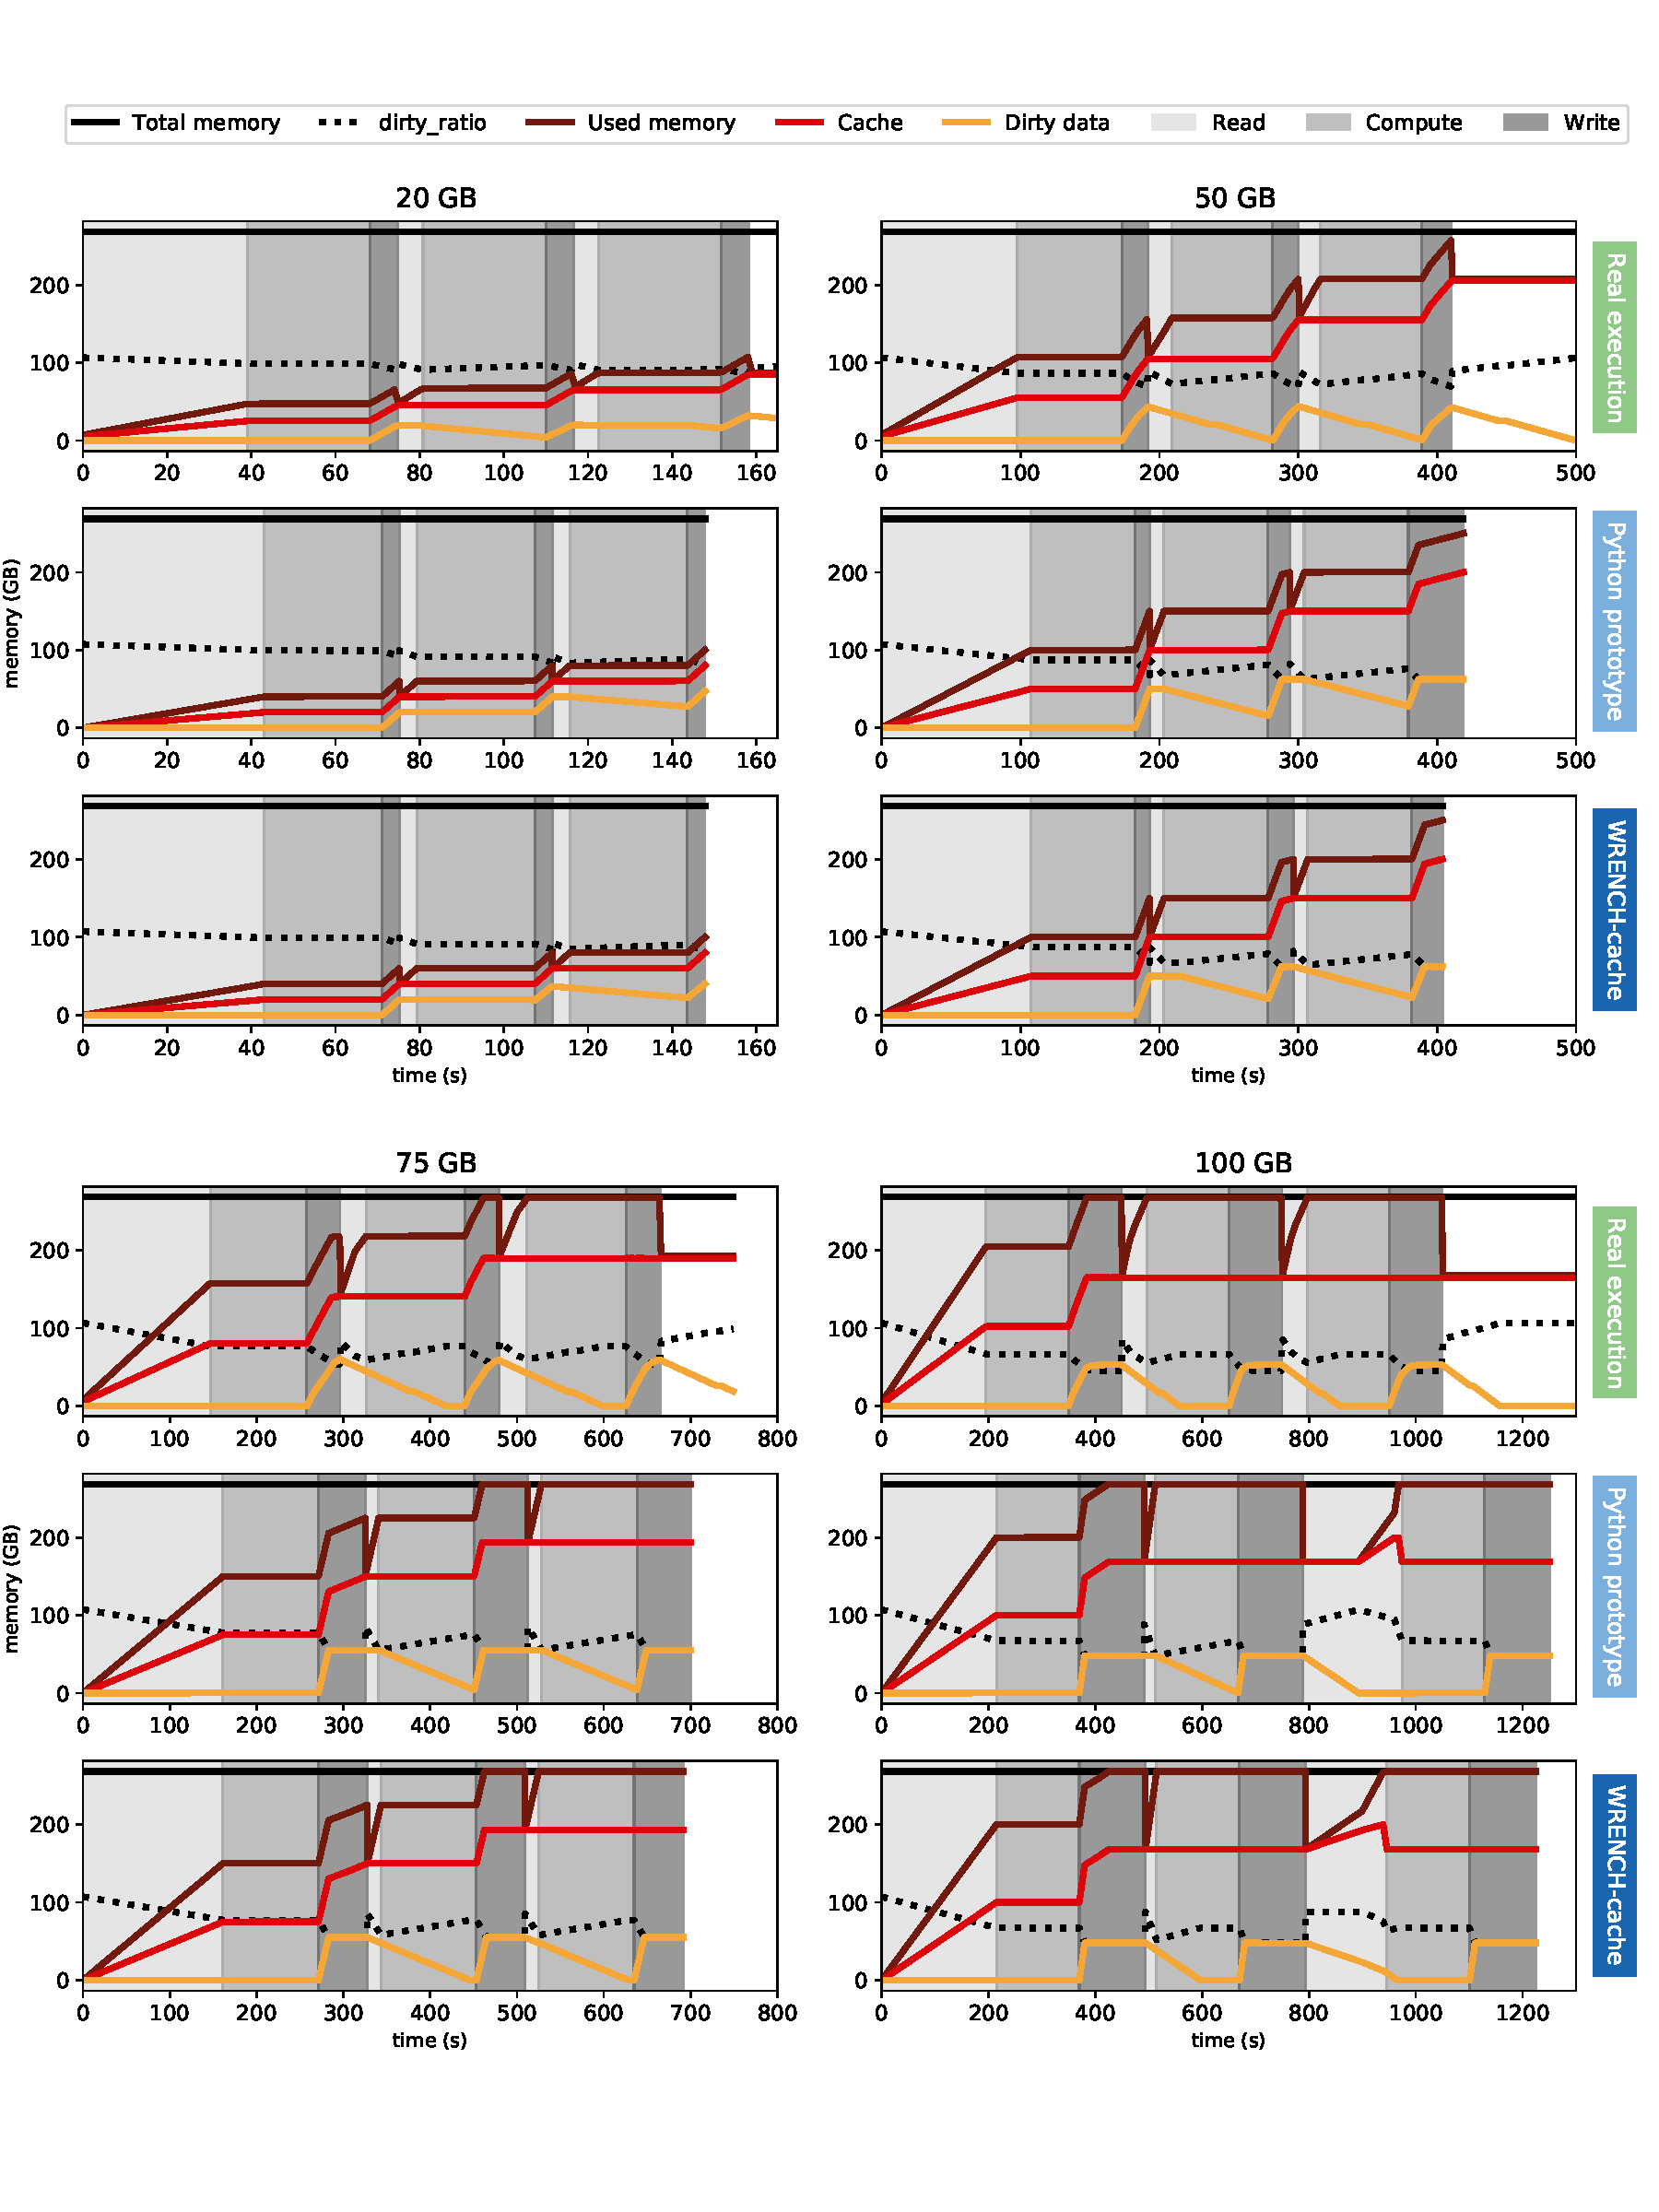
\includegraphics[width=\linewidth]{figures/single_memprof_full.pdf}
%      \vspace*{-0.7cm}
      \caption{Single-threaded application memory profiles with different file sizes}
%      \vspace*{0.5cm}
      \label{fig:single_memprof}
\end{figure*}

Simulated memory profiles with different file sizes were highly consistent 
with the real ones (Figure~\ref{fig:single_memprof}). 
With 20~GB, 50~GB and 75~GB files, memory profiles almost exactly matched 
the real ones, although dirty data seemed to be flushing faster in real life than 
in simulation.
With 50~GB files, this slower dirty data flushing led to a larger amount of 
dirty data after Read~3 in simulation than in reality, which caused longer write 
time of Write~3 when less data was written to cache. 
The simulated memory profiles of 75~GB files were also matched with 
the real ones, except that there were plateaus in file writes, which also 
induced longer write time as in Read~3 with 50~GB files.
With 100~GB files, used memory reached total memory during the first write, 
triggering dirty data flushing, and dropped back to cached memory 
when application tasks released anonymous memory. 
Simulated cached memory was highly consistent with real values, except toward 
the end of Read~3 where it slightly increased in simulation but not in reality. 
This occurred due to the fact that after Write~2, File~3 was only partially
cached in simulation whereas it was entirely cached in the real
system. Thus, Read~3 happened in memory in the real system, but part of 
File~3 was read from disk in simulation, leading longer simulated read time. 
In all cases, dirty data remained under the dirty ratio as
expected. The Python prototype and \wrench-cache exhibited nearly
identical memory profiles, which reinforces the confidence in our
implementations.

\begin{figure*}[!h]
    \centering
       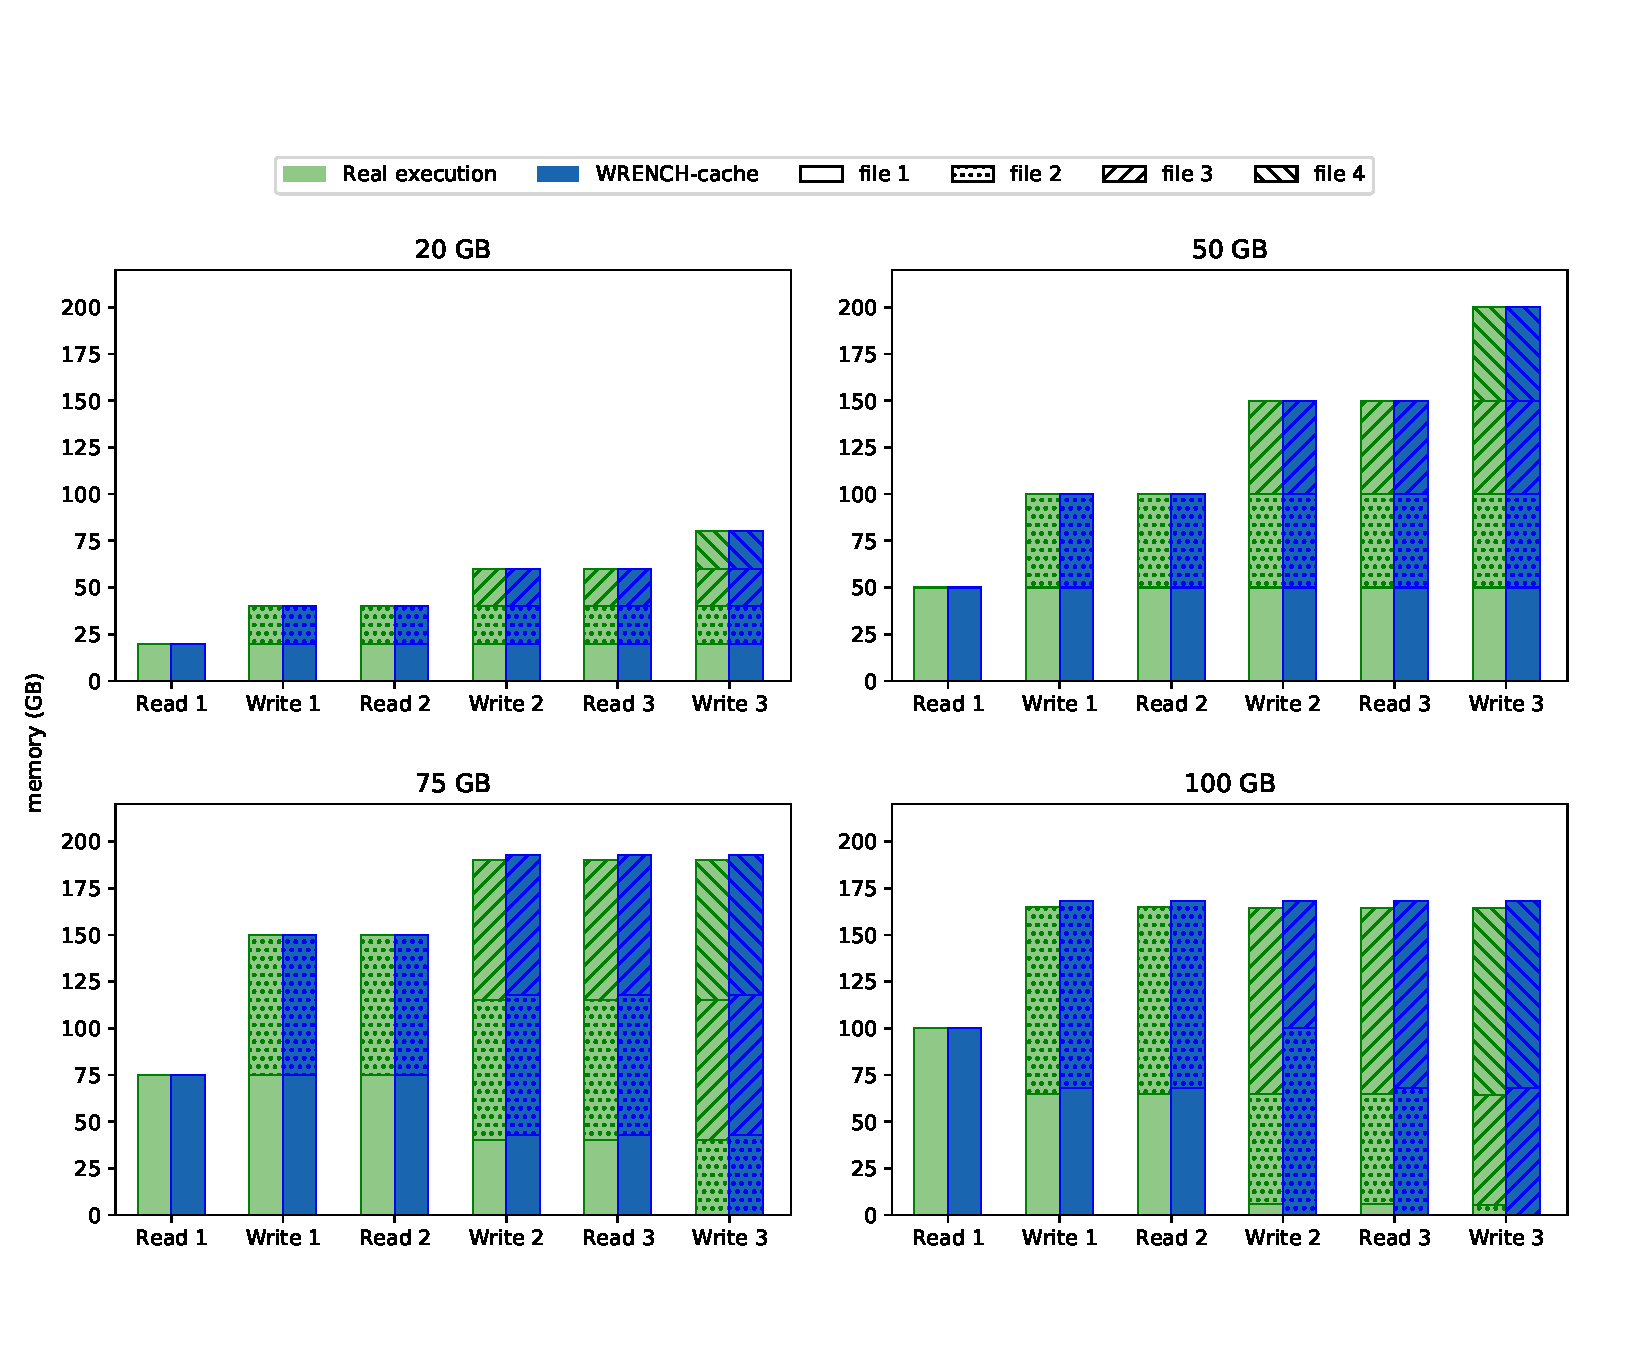
\includegraphics[width=\linewidth]{figures/cached_files_full.pdf}
       \caption{Cache contents \emph{after} single-threaded application I/O operations}
    % \textcolor{red}{Update real results of 20GB}}
       \label{fig:single_cache}
\end{figure*}

The content of the simulated memory cache was also highly consistent with 
reality (Figure~\ref{fig:single_cache}). With 20~GB and 50~GB files, 
the simulated cache content exactly matched reality, since all files fitted 
in page cache. With 75~GB files, the amount of File~1 cached after Write~2 
and Read~3 in reality were slightly less than the simulated amount, but 
the cached data amount of files in simulation matched reality in overall.
With 100~GB files, a slight discrepancy was observed after Write~2, 
which explains the simulation error previously mentioned in Read~3. 
In the real execution indeed, File~3 was entirely cached after Write~2, 
whereas in the simulated execution, only a part of it was cached. 
This was due to the fact that the Linux kernel tends to not evict pages that
belong to files being currently written (File~3 in this case), which we could 
not easily reproduce in our model.

\FloatBarrier

\subsection{Concurrent applications (Exp 2)}

Figure~\ref{fig:multi_local} presents the average read and write time 
of each pipeline in the concurrent applications experiment.
As is shown in the figure, the page cache model notably reduced \wrench's 
simulation error for concurrent applications executed with local I/Os. 
For reads, \wrench-cache slightly overestimated runtime, due to the 
discrepancy between simulated and real read bandwidths mentioned before, 
in which simulated read bandwidth is slower than the real one.
For writes, \wrench-cache retrieved a plateau similar to the one observed 
in the real execution. This was marked with the limit at which all data of 
pipelines could still fit into the page cache. Beyond this limit, the page cache 
was saturated with dirty data and needed flushing.

\begin{figure*}[!h]
    \begin{subfigure}{\linewidth}
        \centering
        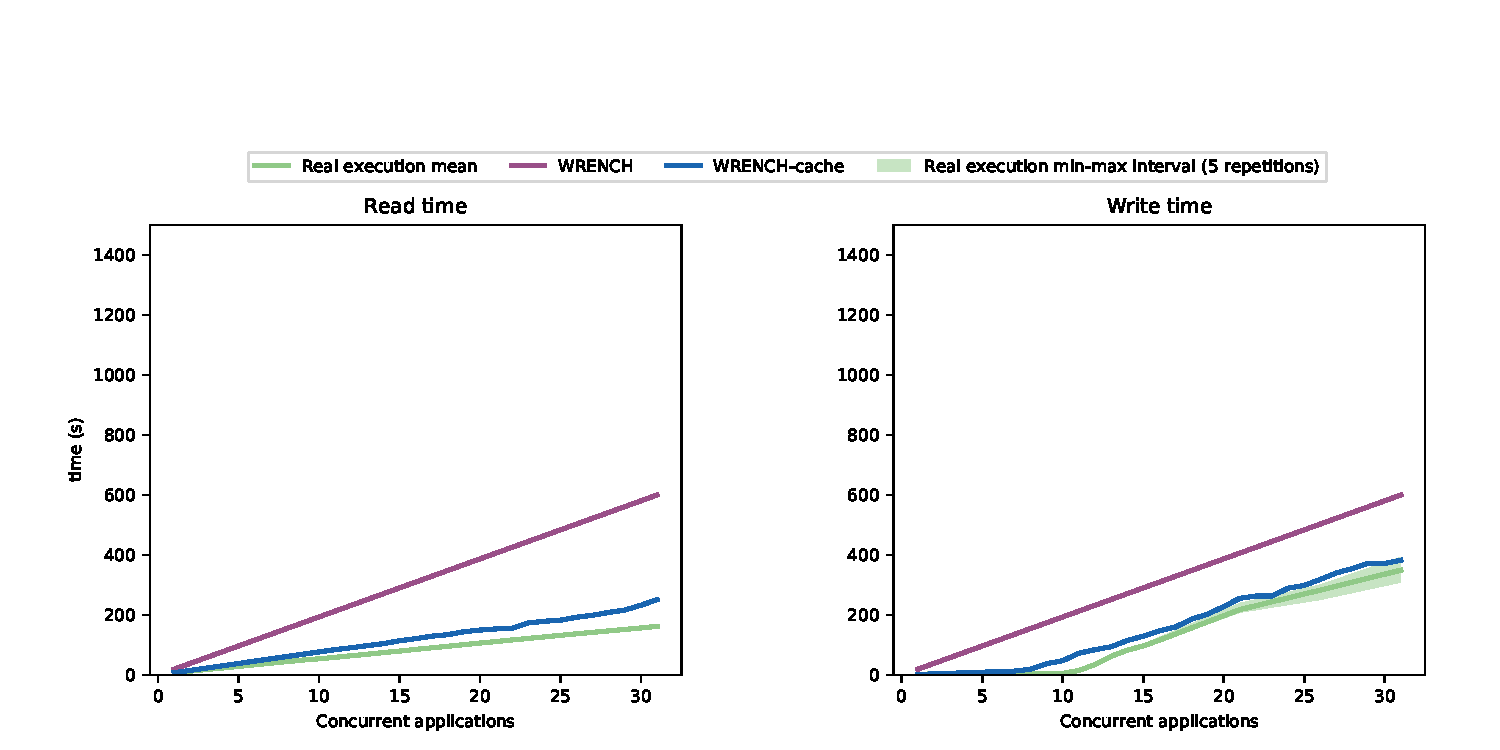
\includegraphics[width=\linewidth]{result/multi/figures/multi_local.pdf}
    \end{subfigure}
    \caption{Results of concurrent applications on local storage with 3~GB files 
    (\textit{Exp 2})}
    \label{fig:multi_local}
\end{figure*}

\FloatBarrier

\subsection{Remote storage (Exp 3)}

Similar to the the previous experiment, the average read and write time 
with concurrent applications on remote storage are illustrated 
in Figure~\ref{fig:multi_nfs}.
The figure shows that page cache simulation importantly reduced 
simulation error on NFS storage as well. 
This manifested only for reads, as the NFS server used writethrough rather 
than writeback cache, which means all write operations happened at disk 
write bandwidth. 
Both \wrench and \wrench-cache
underestimated write times due to the discrepancy between
simulated and real bandwidths mentioned previously. 
For reads, this discrepancy only impacted the results beyond 22
concurrent applications. Before this threshold, most reads resulted in 
cache hits, while after this threshold, \wrench-cache did not accurately 
simulate data flushing and cache eviction, similar to what we observed in 
the single-threaded experiment with 100~GB files and leading to 
less cache hits and more data read from disk in simulation than in reality. 

\begin{figure*}[!h]
    \begin{subfigure}{\linewidth}
        \centering
        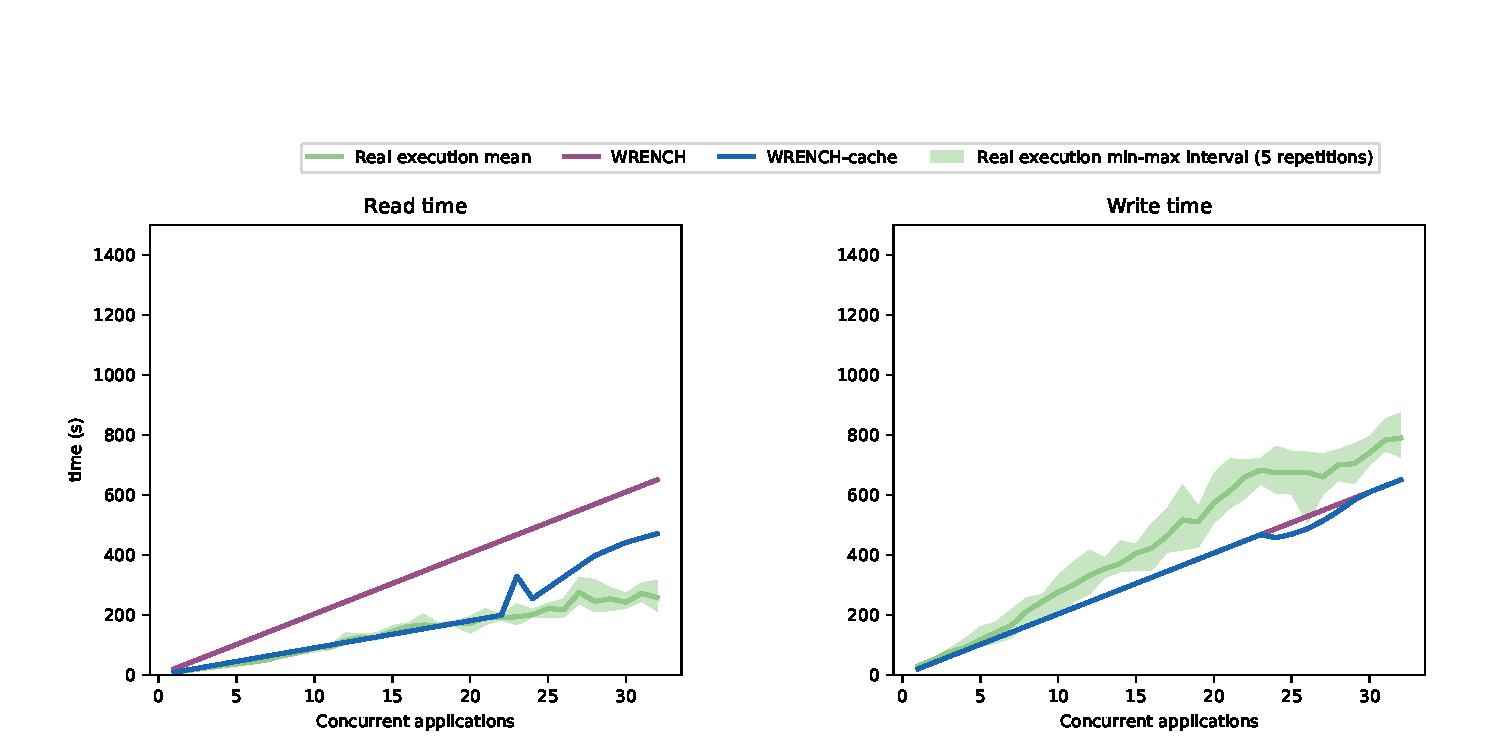
\includegraphics[width=\linewidth]{result/multi/figures/multi_nfs.pdf}
    \end{subfigure}
    \caption{Results of concurrent applications on NFS with 3~GB files 
    (\textit{Exp 3})}
    \label{fig:multi_nfs}
\end{figure*}

\FloatBarrier

\subsection{Real application (Exp 4)}
Similar to the synthetic application, simulation errors of the real 
application were substantially reduced by the WRENCH-cache simulator 
compared to WRENCH (Figure~\ref{fig:nighres}). 
On average, errors were reduced from 337~\% in WRENCH to 47~\% in 
WRENCH-cache. 
The first read happened entirely from disk and was therefore 
very accurately simulated by both WRENCH and WRENCH-cache.

\begin{figure*}[!ht]
    \begin{subfigure}{0.95\linewidth}
        \centering
        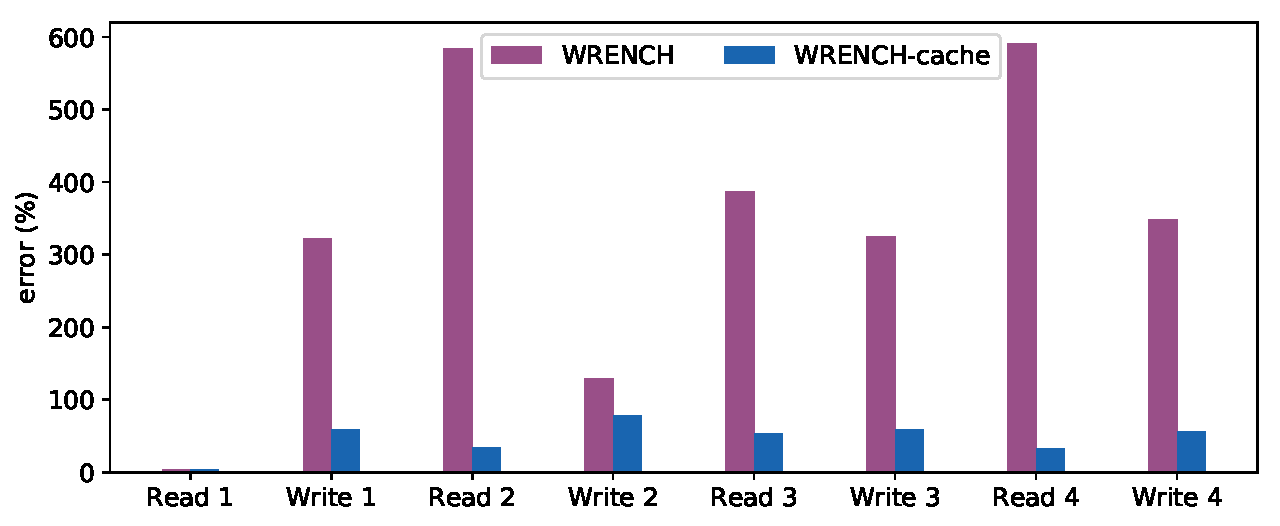
\includegraphics[width=\linewidth]{result/nighres/figures/nighres_errors.pdf}
    \end{subfigure}
    \caption{Real application results (\textit{Exp 4})}
    \label{fig:nighres}
\end{figure*}

\FloatBarrier

\subsection{Simulation time}

As is the case for \wrench, simulation time with \wrench-cache scales
linearly with the number of concurrent applications
(Figure~\ref{fig:multi_time}, p \textless $10^{-24}$). However, the page
cache model substantially increases simulation time by
application, as can be seen by comparing regression slopes in
Figure~\ref{fig:multi_time}. Interestingly, \wrench-cache is faster with 
NFS I/Os than with local I/Os, most likely due to the use of writethrough
cache in NFS, which bypasses flushing operations.

\begin{figure}[!h]
    \begin{subfigure}{\columnwidth}
        \centering
        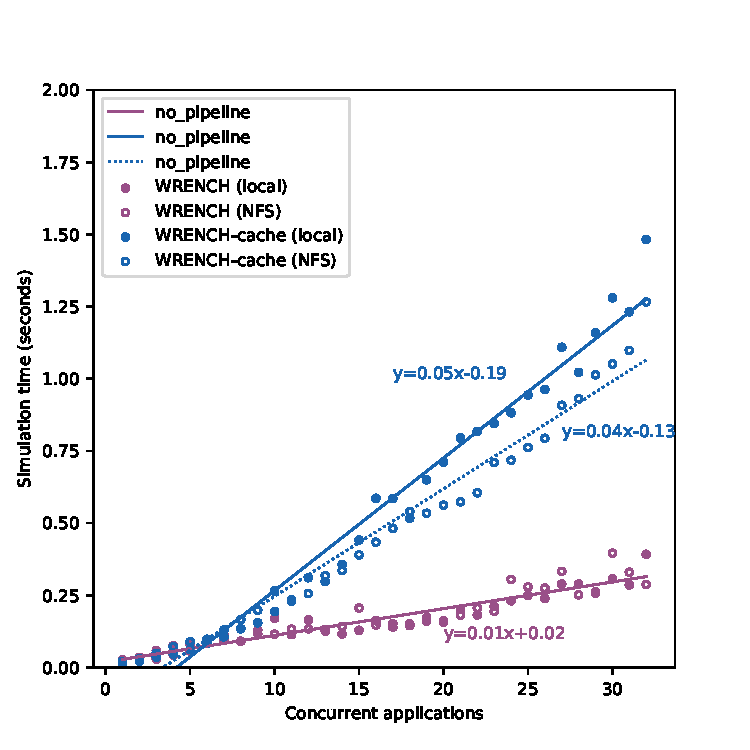
\includegraphics[width=0.8\linewidth]{result/multi/figures/simulation_time.pdf}
    \end{subfigure}
    \caption{Simulation time comparison. \wrench-cache scales
    linearly with the number of concurrent applications, albeit
    with a higher overhead than \wrench.}
    \label{fig:multi_time}
\end{figure}